% First line in your LaTeX file should be the \documentclass{} command.
% 'article' is good for our purpose of writing a report.
% You can find a full list
\documentclass{article}

% Language setting
% Replace `english' with e.g. `spanish' to change the document language
\usepackage[english]{babel}

% Set page size and margins
% Replace `letterpaper' with `a4paper' for UK/EU standard size
\usepackage[letterpaper,top=2cm,bottom=2cm,left=1cm,right=1cm,marginparwidth=1.75cm]{geometry}

% Useful packages
\usepackage{amsmath}
\usepackage{graphicx}
\usepackage[colorlinks=true, allcolors=blue]{hyperref}
\usepackage{multicol}
\usepackage{fancyhdr}
\usepackage{caption}
\usepackage{braket}
\usepackage{mathtools}

\title{\textbf{Randomized Benchmarking}}
\author{Kale Chen, Henry Zhang}
\date{Apr. 21, 2026}

\begin{document}

\pagestyle{fancy}
\fancyhead[R]{Kale Chen, Henry Zhang}
\fancyhead[L]{Randomized Benchmarking}

\maketitle

\begin{multicols}{2}

\section{Introduction}

In quantum computing, we are often concerned with errors on qubits, since qubits are very sensitive to noise and easily lose their state. Randomized benchmarking is an analytical technique intended to isolate the error introduced by gate operations, which degrade the state by direct interaction. This report details our study of single qubit Clifford gate operations and their error rates through a randomized benchmarking method performed on IBM QPUs through the Qiskit API.

\subsection{Theory}
\subsubsection{Single Qubit Clifford Gates}
For this study we are broadly concerned with randomized benchmarking of Clifford gate operations, which map Pauli operators to other Pauli operators. We like these in quantum computing because they define the set of gate operations that keep a code within the Pauli group. We focus on single qubit Clifford gates, which can all be constructed from the $H$ and $S$ gates and their adjoints. There are 24 unique single qubit Clifford gates, corresponding to unique 90 degree rotations of the axes of the Bloch sphere.
\subsubsection{Model}
Beginning with an initial state $\ket{\psi}$, we can expect some error to accumulate on this state after many Clifford gate operations. Taking a sort of informal argument, say the probability of an error occuring after a single Clifford gate $U$ acting on $\ket{\psi}$ is $p$, after $m$ gates, the possible states can be represented with the binomial expansion:
\[(pU + (1-p)I)^m \ket{\psi} = \sum_{i=0}^m {m\choose i} p^i U^i (1-p)^{m-i} I^{m-i} \ket{\psi}\]
If $p<<1$, then the main contribution to the probability of measuring the correct state is given by the first term, after which every subsequent term is exponentially smaller. 
\[F \approx (1-p)^m\]
Thus, seeing the exponential behavior of this kind of problem, we can model the fidelity as a function of the number of Clifford gate operations $m$ as:
\[F(m) = A (1-p)^m + B\]
As $m$ grows large and the qubit accumulates more errors, however, then larger order terms become more significant, and the state should reach a maximally random state, where there is a half probability of measuring the correct state. Thus, we would expect $B$ to be very close to 0.5. There are some more nuances to this, such as the fact that Clifford errors do not always ``flip'' the state (180 degree rotations), can be any permutation of 90 degree rotations. We will see that an exponential is still sufficient to model the mechanism.

\section{Methodology}
To do randomized benchmarking, we created a circuit with some length of random Clifford gates and their inverses applied to a single qubit initialized in the $\ket{0}$ state. We then measured the qubit after 1000 shots of the circuit and recorded the counts of the $\ket{0}$ and $\ket{1}$ states, which we used to calculate an estimate for the fidelity of this specific Clifford sequence. Since we are preparing the state in the $\ket{0}$ state, we take the fidelity to be the number of measured $\ket{0}$ states divided by the total number of shots (1000 for our case):
\[F = \frac{N_0}{N_0 + N_1} = \frac{N_0}{1000}\]
We performed this process for Clifford sequences of lengths 1, 2, 5, 10, 20, 50, 100, 200, and 500, each with 10 different random Clifford sequences for a total of 90 data points. We would have liked to take more data but we are ultimately limited in usage by IBM.

To analyze, we will take an average of the fidelity estimates for each Clifford sequence length, and fit these averages to our exponential model. For uncertainty treatment, we will use the standard error of the mean, adjusted by a factor to account for potential variation in native gate length, discussed in the next section. This is necessary due to our low volume of data.   

\subsection{Additional Considerations}
Abstractly, there is no distinction between each of the single qubit Clifford gates, and we can treat them as equivalent in the sense that they introduce error with the same probability. In a real circuit, however, each single qubitClifford gate must still be constructed from a specific sequence of gates, ranging in total length from 1 to 4. This means that, even with the assumption that all the native gates have the same error rate, the error rate of each Clifford gate will be different according to its construction length. Over long sequences, this behavior averages out, but for short sequences, careful uncertainty treatment is necessary, as individual sequences that happen to contain significantly different gate lengths will appear to have more deviated fidelity estimates.

Furthermore, on IBM's hardware, every gate is realized by a sequence of hardware level operations: $R_Z(\pi)$, $R_Z(\pi/2)$, $X$, and $\sqrt{X}$. For example the $H$ gate is constructed as:
\[H = R_Z(\pi/2) \sqrt{X} R_Z(\pi/2)\]
This adds even more complexity to each Clifford gate's true length. To account for this, we introduce a factor which describes the deviation of true gate length for the 10 samples for each Clifford sequence length $m$. This factor is calculated as the standard error of the length, meaning the scaling factor $\sqrt{m}$ will impact the uncertainty of shorter sequences more. As previously mentioned, this is expected as longer sequences should exhibit more averaged behavior. As a note, this uncertainty treatment is implicit in the Clifford sequence length, it is just simply 0 because the lengths are defined to be equal.


\section{Results}
First, we did a quick comparison of clifford sequence length and hardware gate length, shown in Figure \ref{fig:clifford_vs_hardware}. For each Clifford sequence length, we have 10 random samples which should differ slightly in their true hardware gate length. At very short sequence lengths, the hardware gate length deviates strongly from the mean, and as sequence length increases, the hardware gate length behavior averages out, shown by the decreasing magnitude of the standard errors. Here the standard error is calculated as
\[SE_L = \frac{\sigma_L}{\sqrt{L}}\]
where $\sigma_L$ is the standard deviation of the hardware gate lengths and $L$ is the mean hardware gate length for the 10 samples. A standard linear fit suggests that on average, there are approximately 4.07 hardware gates per Clifford gate.



Now that we have the standard error contribution from hardware gate length, we can incorporate this into our uncertainty treatment for the fidelity estimates. For each Clifford sequence length, we compute a fidelity estimate for each of the 10 samples, then take the standard error in the typical way:
\[SE_F = \frac{\sigma_F}{\sqrt{10}}\]
The combined standard error is then calculated as the root sum of squares of the normalized standard errors:
\[SE = \sqrt{\left(\frac{SE_F}{\bar{F}}\right)^2 + \left(\frac{SE_L}{\bar{L}}\right)^2}\]
where the bars indicate mean. These combined standard errors are then used to fit the exponential model, shown in Figure \ref{fig:fit}. We can see the exaggerated error on the Clifford sequence of length 1, which quickly dampens down as the sequence length increases. Overall we obtain a strong fit, with reduced chi square of 1.03. The parameters are: 
\[A = 0.489 \pm 0.009\] 
\[B = 0.487 \pm 0.001\] 
\[p = 0.0113 \pm 0.0002\] 
The amplitude terms $A$ and $B$ are both close to the expected values of 0.5. The probability term $p$ indicates that every Clifford gate has on average a 0.0113 probability of introducing error. As discussed previously, this is a generous estimate, as our model does not account for errors that may return the state to the correct state, or errors that partially twist the state but can still be measured correctly.



We might also be interested in a similar fit on the hardware gate length, shown in Figure \ref{fig:hardware_fit}. This fit is over all 90 samples, so we should expect clusters of points centered on the approximately 4.07 times our $m$ values for each Clifford sequence length, and we obtain a probability of error per hardware gate of 
\[p = 0.0028 \pm 0.0052\]
Here the uncertainty is quite large due to the fit over all 90 samples, but the predicted value agrees very well with what we would expect from our fit on the Clifford sequence length:
\[p = 1 - (1-0.0113)^{1/4.07} = 0.00279\]



\section{Conclusion}
Our results and analysis finds the expected behavior as the Clifford sequence length increases. We offer a metric to quantify the error rate per Clifford or hardware gate. We obtain a $p = 0.0113 \pm 0.0002$ probability of error per Clifford gate implemented on a single qubit on an IBM QPU. 

\subsection{Suggestions for Future Work}
It is necessary to try similar analysis on different qubits to compare the behavior across different qubits on the same hardware. It is not true that the error rate will be the same for all qubits, and it is important to get an idea of what the distribution of error rates across many qubits looks like. We didn't get to this part because we were exhausting our QPU usage, but it wouldn't take much more effort since we have the scripts for analysis already written.

It may also be worthwhile to investigate outliers in the data to see if they reveal anything about the underlying noise of this kind of hardware. Even with long sequences, there is still deviation in the relative frequencies of each gate that constitutes a single Clifford gate. These deviations in relative frequencies may be the cause of overall fidelity deviations.

In general, with this kind of study, there are many underlying assumptions that we make to abstract the problem into a simpler model, and there are many hardware considerations that we should account for. Another direction to take is to bias Clifford selection to favor those including a specific gate, such as the $Y$ gate, which is high weight in terms of hardware gate length.

\end{multicols}
\begin{figure}[h]
    \centering
    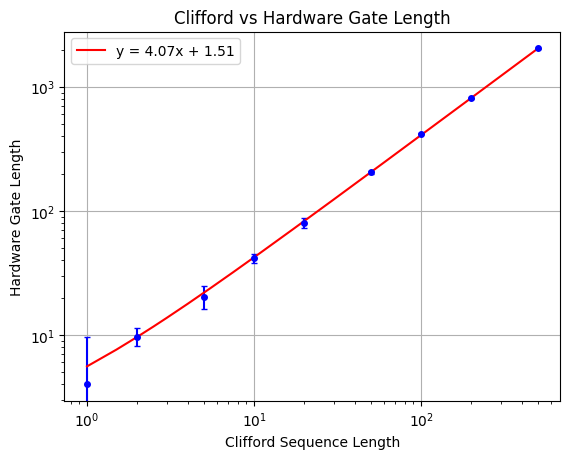
\includegraphics[width=0.7\textwidth]{cliffordhardware.png}
    \caption{Comparison of Clifford sequence length and hardware gate length}
    \label{fig:clifford_vs_hardware}
\end{figure}
\begin{multicols}{2}

\end{multicols}
\begin{figure}[h]
    \centering
    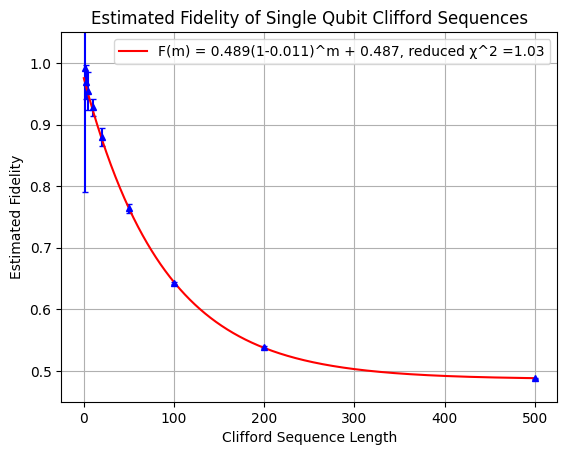
\includegraphics[width=0.7\textwidth]{fidelity.png}
    \caption{}
    \label{fig:fit}
\end{figure}
\begin{multicols}{2}

\end{multicols}
\begin{figure}[h]
    \centering
    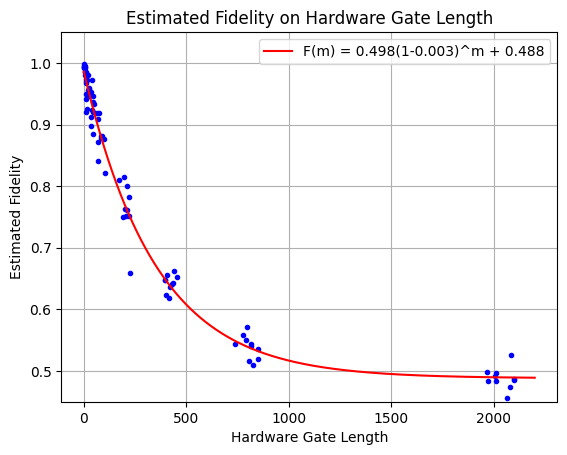
\includegraphics[width=0.7\textwidth]{fidelityhardware.png}
    \caption{}
    \label{fig:hardware_fit}
\end{figure}
\begin{multicols}{2}


\end{multicols}

\end{document}